\documentclass[11pt,a4paper]{article}
\usepackage[margin=17mm,headheight=14pt,headsep=6mm,footskip=9mm]{geometry}
\usepackage{amsmath,amssymb,booktabs,array,tabularx,xcolor,tikz,fancyhdr}
\usepackage[colorlinks=true,linkcolor=blue!45!black,urlcolor=blue!45!black]{hyperref}
\definecolor{ink}{HTML}{173247}
\definecolor{teal}{HTML}{167D8D}
\definecolor{gold}{HTML}{AB681F}
\pagestyle{fancy}\fancyhf{}
\fancyhead[L]{\small\textcolor{ink}{BOUNDARY-10 \quad Decagon and outer closure}}
\fancyhead[R]{\small 16 October 2026}
\fancyfoot[L]{\small Exploratory mathematics \enspace | \enspace GPT / owner discussion}
\fancyfoot[R]{\thepage/4}
\setlength{\parindent}{0pt}\setlength{\parskip}{5pt}
\setlength{\abovedisplayskip}{6pt}\setlength{\belowdisplayskip}{6pt}
\newcommand{\head}[1]{\vspace{3pt}{\large\bfseries\color{ink}#1}\par}
\newcommand{\tagline}[1]{\textbf{\textcolor{teal}{#1}}}
\newcommand{\R}{\mathbb R}
\newcommand{\conv}{\operatorname{conv}}
\newcommand{\uvec}{\boldsymbol u}
\begin{document}
{\LARGE\bfseries\color{ink}Can a decagon close the Tri-Octagon?}\par
\textbf{Finding.} A decagonal prism is a valid optional enclosure, but tenfold geometry does not follow from the welded shell. The simplest intrinsic round enclosure is its existing vertex circumsphere, which is also the unique smallest enclosing sphere. Neither construction derives the proposed $T=\pi e\phi$, $B=10$ or an outside remainder. Here $\phi=(1+\sqrt5)/2$ and $e=\exp(1)$.

\head{1. Reused exact geometry and scope}
Paper C v1.0.1 [C, \S\S2--9] fixes three regular octagonal panels of flat-to-flat width $w>0$, edge $s=(\sqrt2-1)w$, folded at $60^\circ$. Their welded surface $S$ has 18 vertices, three faces, and two \emph{nonplanar} nine-edge rims. It is an annulus, with symmetry $D_{3h}$; it does not bound a solid by itself. Its axial projection is the perimeter of an equilateral triangle $K$ of side $w$, and $|z|\leq w/2$.

The accepted SHAPES atlas [A, pp.3,11--15,19] already supplies polygon metrics, the vertex-sphere radius, the decagon comparison row, and support-normal interleaving. Those results are reused, not reopened. The historical ninth identity, the nine-edge native rim, and the author's new tenth-boundary proposal remain three different notions. The new $T$ is unrelated by definition to the old two-input selector also named $T$.

\head{2. Exact regular-decagon identities}
\tagline{Definition.} A filled regular decagon has vertices
\[
 v_k=c+R\bigl(\cos(\eta+k\pi/5),\sin(\eta+k\pi/5)\bigr),\quad k=0,\ldots,9,
\]
with $R>0$; its boundary is the ten-edge cycle. The central angle and exterior turn are $36^\circ$, each interior angle is $144^\circ$, and the interior-angle sum is $1440^\circ=8\pi$. Its planar symmetry is $D_{10}$ of order 20 (ten rotations and ten reflections), not a group of order 10.

\tagline{Derivation.} Put $x=2\cos36^\circ>0$. From $\cos108^\circ=-\cos72^\circ$ and the double/triple-angle identities [N],
\[
 x^3-3x=2-x^2,\qquad (x+2)(x^2-x-1)=0.
\]
Thus $x=\phi$, $\sin18^\circ=\cos72^\circ=1/(2\phi)$, and
\[
 \cos18^\circ=\frac{\sqrt{10+2\sqrt5}}4,\qquad
 t:=\tan18^\circ=\frac1{\sqrt{5+2\sqrt5}}.
\]
Bisecting a centre-side triangle gives the side $\ell$, apothem $a$, perimeter $P$ and filled area $A$:
\[
 \ell=2R\sin18^\circ=\frac R\phi=2at,\quad a=R\cos18^\circ,
 \quad P=10\ell,\quad A=\frac{Pa}{2}=10a^2t.
\]
Every chord is $d_j=2R\sin(j\pi/10)$, $1\leq j\leq5$. In particular $d_3=\phi R=\phi^2\ell$ and $d_5=2R$. The scale-free ratios include $R/\ell=\phi$, $P/R=10/\phi$, $A/R^2=5\sin36^\circ$, and $4\pi A/P^2=\pi/(10t)$. A similar decagon scales lengths by $\lambda$ and areas by $\lambda^2$; its side count stays 10. None of these identities supplies a physical unit.

\newpage
\head{3. Octagonal and decagonal angles are different data}
The existing comparison convention is $a=w/2$ [A]; it is not an enclosure rule.
\begin{center}\renewcommand{\arraystretch}{1.2}
\begin{tabular}{@{}lcc@{}}\toprule
Quantity & Regular octagon & Regular decagon\\\midrule
Central angle / exterior turn & $45^\circ$ & $36^\circ$\\
Interior angle & $135^\circ$ & $144^\circ$\\
Side divided by $w$ & $\sqrt2-1\approx0.414214$ & $t\approx0.324920$\\
Circumradius divided by $w$ & $[2\cos(\pi/8)]^{-1}\approx0.541196$ & $[2\cos(\pi/10)]^{-1}\approx0.525731$\\
Area divided by $w^2$ & $2(\sqrt2-1)\approx0.828427$ & $5t/2\approx0.812299$\\\bottomrule
\end{tabular}\end{center}
The angle difference is $9^\circ$. For \emph{co-centred, coplanar} aligned direction grids, $45^\circ=5(9^\circ)$ and $36^\circ=4(9^\circ)$ generate a 40-direction refinement; their common rotations form $C_2$. This is arithmetic, not a new folded-shell symmetry. In particular, the shell's $60^\circ$ fold and $120^\circ$ normal separation are not polygon exterior turns.

\tagline{Symmetry obstruction.} A regular axial decagon cannot be invariant under the shell's $120^\circ$ rotation: $120/36=10/3$ is not an integer. A unique enclosure selected solely by the unlabelled shell through a symmetry-respecting rule must preserve that rotation. Therefore it cannot have a regular decagonal axial cross-section. Containment is still possible; it needs an additional orientation choice. The combined shell and decagonal enclosure have no nonidentity common rotation about this axis, since $C_3\cap C_{10}=\{1\}$.

\head{4. Spatial enclosures already supported by the geometry}
Use Paper C's centre $o=(0,\sqrt3w/6,0)$. Its three panel centres lie at perpendicular distance $p=w/(2\sqrt3)$ from $o$. Each panel has circumradius $R_8=w/[2\cos(\pi/8)]$. Reusing [A, p.11], every one of the 18 vertices lies on
\[
 \boxed{\quad \|x-o\|=\rho,\qquad
 \rho^2=p^2+R_8^2=w^2\left(\frac{13}{12}-\frac{\sqrt2}{2}\right).
 \quad}
\]
\tagline{New enclosure consequence, with proof.} The closed ball contains every panel: each panel is the convex hull of its vertices and a ball is convex. The vertex average is $o$ by the threefold and horizontal-reflection symmetries. For any proposed centre $c$,
\[
 \frac1{18}\sum_{i=1}^{18}\|v_i-c\|^2=\rho^2+\|c-o\|^2.
\]
Any ball containing all vertices therefore has squared radius at least this average. The ball centred at $o$ attains radius $\rho$; any other centre needs a strictly larger radius. This proves the unique smallest enclosing ball, not merely a convenient spherical bound.

Two other exact constructions are useful. The solid $K\times[-w/2,w/2]$ is a triangular-prism envelope fixed by the known projection and height. The convex hull $\conv(S)$ is the unique smallest \emph{convex set} containing the shell; choosing convexity is a convention, though the hull then needs no free parameter. Neither is tenfold. These envelopes contain $S$ but touch it; strictly positive clearance requires an additional specified distance. They are mathematical reference constructions, not added kernel surfaces or material caps.

\newpage
\head{5. A precise optional tenfold enclosure}
Let $r_c=w/\sqrt3$ be the triangle circumradius. With coordinates $r=(x,y)-o_{xy}$, define the filled planar decagon and the solid prism
\[
 D_{10}(a,\theta)=\{r:\uvec(\theta+j\pi/5)\cdot r\leq a,\ 0\leq j<10\},
 \qquad \uvec(\gamma)=(\cos\gamma,\sin\gamma),
\]
\[
 E_{10}(a,\theta)=\{(o_{xy}+r,z):r\in D_{10}(a,\theta),\ |z|\leq w/2\}.
\]
Here $\theta$ is a \emph{side-normal} angle. A planar decagon alone bounds only a planar region or projection. The prism is three-dimensional; its complete boundary has ten rectangular sides and two decagonal caps, hence \emph{12 faces}, not ten. Omitting the caps leaves an open lateral surface.

\tagline{Exact containment criterion.} Write the three triangle corner directions as $\alpha_k=\alpha_0+2\pi k/3$. The least apothem for a fixed orientation is
\[
 a_*(\theta)=r_c\max_{\substack{0\leq j<10\\0\leq k<3}}
          \cos(\theta+j\pi/5-\alpha_k).
\]
This is necessary because the shell contains the three seam footprints. It is sufficient because all projected shell points lie on $\partial K$, and linear inequalities holding at the three corners hold throughout their convex hull $K$.

\tagline{Bounded optimization, not a fit to a target constant.} The angle differences $36j-120k$ cover every multiple of $12^\circ$ modulo $360^\circ$: after division by 12 the residues $3j-10k$ are all distinct modulo 30. The closest difference to a multiple of $360^\circ$ has magnitude $d\in[0,6^\circ]$. Consequently $a_*=r_c\cos d$ and
\[
 \min_{\theta}a_*(\theta)=r_c\cos6^\circ,
 \qquad \theta-\alpha_0=6^\circ\pmod{12^\circ}.
\]
This minimum holds \emph{only for decagons centred on the native axis}, with free orientation. It is not a claim about translated or tilted enclosures. There are three equally good orientations modulo the decagon's $36^\circ$ period, exchanged by the shell's threefold rotation; the shell selects none uniquely. Alternatively $a=r_c$ works at every orientation, but is larger. The atlas's $a=w/2$ decagon is too small for this centred enclosure, since $r_c\cos6^\circ>w/2$.

\begin{center}
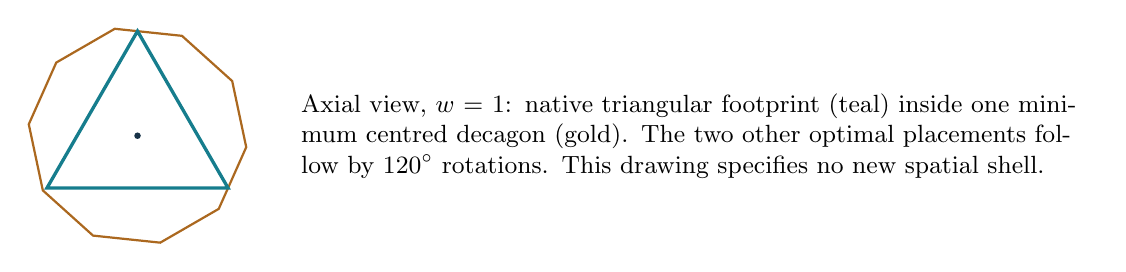
\begin{tikzpicture}[scale=2.3]
\def\rr{0.5773502692}\def\aa{0.5741874840}
\pgfmathsetmacro{\Rdec}{cos(6)*\rr/cos(18)}
\draw[gold,thick] (30:\Rdec) \foreach \a in {66,102,138,174,210,246,282,318,354} {--(\a:\Rdec)} --cycle;
\draw[teal,very thick] (90:\rr)--(210:\rr)--(330:\rr)--cycle;
\fill[ink] (0,0) circle(0.018);
\node[anchor=west,text width=10cm,align=left,font=\small] at (0.85,0.0) {Axial view, $w=1$: native triangular footprint (teal) inside one minimum centred decagon (gold). The two other optimal placements follow by $120^\circ$ rotations. This drawing specifies no new spatial shell.};
\end{tikzpicture}
\end{center}
Using the accepted support-normal theorem [A, p.19], two equal-apothem pentagons offset by $36^\circ$ intersect in a decagon. That introduces pentagonal data independently. Combining a decagon with its $120^\circ$ and $240^\circ$ rotations by \emph{intersection} instead produces a regular 30-gon. Thirty, the least common multiple of 3 and 10, permits both rotations; it is not a reason to adopt a 30-sided boundary.

\newpage
\head{6. Adopted conventions for $T$, $B$ and $\Delta$}
The author's proposed numbers are consistent as dimensionless scalars:
\[
 T=\pi e\phi\approx13.8175802272,\qquad B=10,\qquad
 \Delta=T-B\approx3.8175802272>0.
\]
Positivity does not need decimal agreement: $\pi>3$, $e>5/2$, $\phi>3/2$ imply $T>45/4>10$. But a number is not a surface. The interpretation depends on the \emph{same specified quantity} being measured for both $T$ and $B$.

\begin{center}\small\renewcommand{\arraystretch}{1.15}
\begin{tabularx}{\linewidth}{@{}p{24mm}X@{}}\toprule
Meaning of $B$ & What follows, and what must be supplied\\\midrule
Side count $n=10$ & Defines combinatorics, not a length, area or volume. Subtracting it from $T$ does not identify a spatial remainder.\\
Length $10L_0$ & Choosing a unit $L_0>0$ and a common radial/linear measure gives $L_T=TL_0$ and $L_T-L_B=\Delta L_0$. It does not choose a shape or prove that these lengths occur in the native geometry.\\
Area or volume & One may adopt $A_0$ or $V_0$ as a common unit. The difference is then an area or volume, not automatically a radial thickness.\\\bottomrule
\end{tabularx}\end{center}
\tagline{Conditional example, not an adopted model.} Concentric spheres of radii $10L_0$ and $TL_0$ have a radial gap $\Delta L_0$, but the intervening volume is $\tfrac{4\pi}{3}L_0^3(T^3-10^3)$. Thus even in this simple model $\Delta$ is not simultaneously a length and a volume. If $T$ means the full radial extent, the radius-10 boundary is a cutoff \emph{inside} that extent, not the final enclosing boundary of the complete object.

\tagline{A natural decagonal normalization.} With side unit $L_0=\ell$, the perimeter satisfies $P/L_0=10$ and the circumcircle has $C/L_0=2\pi\phi$. Thus $T=(e/2)(C/L_0)$. Identifying $T$ with a circular perimeter would require the extra radius $(e/2)R$; that dilation is not forced by the shell and is not adopted here. A perimeter difference is not outside area or volume. Alternatively, any radius $r_b$ can be renamed 10 by taking $L_0=r_b/10$, but requiring $r_T/r_b=T/10$ is an independent geometric assumption. No parameters were fitted to either target. No claim about the algebraic or transcendental status of $\pi e\phi$ is needed.

\head{7. Unresolved relationships and recommendation}
\textbf{Recursive closure is separate.} A closed polygonal path, a closed surface, and closure of an operation are different statements. A tenth-step return would require a state/shape space $X$, an exact map $F:X\to X$, and a condition such as $F^{10}(x)=x$ (with $F^k(x)\ne x$ for $1\leq k<10$ if the period is exactly ten). No such geometric successor map was recovered by SHAPES-01 [S, \S\S3,8; A, p.21]. Adding a decagon neither defines it nor repairs that historical gap.

\textbf{Still unresolved:} what quantity ``total tensor scale'' measures; whether 10 is a count or a metric value; what set lies outside which set; the measure assigned to that remainder; and any map linking the historical ninth identity to a new closing operation. A scalar does not specify a tensor's space, components, norm or transformation rule.

\textbf{Recommended discussion candidate:} the unique minimum enclosing sphere, if the aim is a neutral outer spatial reference; $\conv(S)$ if a tight convex polyhedral envelope is preferred. Retain the centred decagonal prism only as an explicitly optional tenfold comparison with its orientation choice disclosed. No evidence here selects tenfold closure as intrinsic, or identifies $\Delta$ with outside matter, energy or a physical field.

{\footnotesize
\textbf{Sources and evidence.} [C] \emph{Exact Geometry of the Folded Tri-Octagon Module}, Paper C v1.0.1, \S\S2--6,9. [S] \emph{SHAPES01 Codex Reconstruction}, 8 Oct 2026, \S\S2--4,8. [A] \emph{SHAPES01 Atlas v0.1}, final local reference, pp.3,11--15,19,21; GPT mathematical acceptance dated 8 Oct 2026, with source-note closeout. [N] NIST DLMF \href{https://dlmf.nist.gov/4.21}{\S4.21}, double/triple-angle identities, accessed 16 Oct 2026. Exact local paths and input hashes accompany the editable source. Existing research suites were not rerun; the added conclusions have written proofs above. Only scalar display arithmetic and document build/layout checks were performed. No simulation, model implementation, source edit, Git write or publication.}
\end{document}
